\subsection{Merge Results:}

Test of Merge Algorithm. The program will plot the {\bfseries\itshape time} that the algorithm takes to sort a 'list' of size {\bfseries\itshape n = 10}.

\begin{figure}[H]
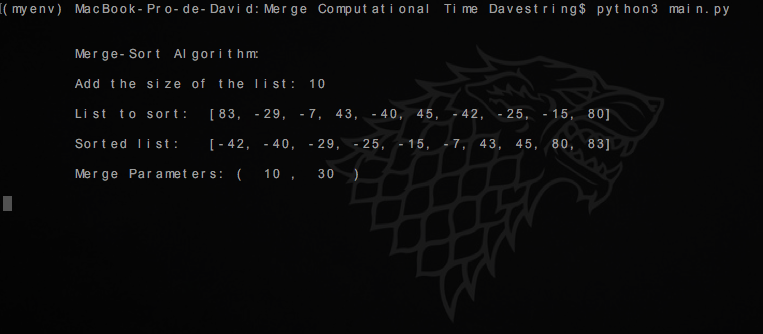
\includegraphics[scale=.6]{console2.png}
\centering \linebreak \linebreak Figure 5.2.0: Console output of Merge algorithm.
\end{figure} \hfill

\begin{multicols}{2}
\begin{figure}[H]
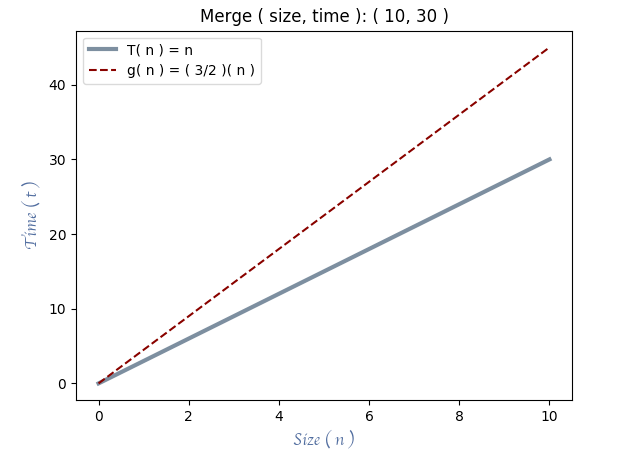
\includegraphics[scale=.45]{plot2.png}
\centering \linebreak \linebreak Figure 5.2.1: Plot of Figure 4.2.0.
\end{figure} 

\begin{center}
\begin{itemize}
\end{itemize}
{\Large
\begin{tabular}[.5cm]{c c c }
\toprule
Size ( n ) & Time ( t ) \\
\midrule
0 & 0 \\
\cmidrule{1-2}
1 & 3 \\
\cmidrule{1-2}
2 & 6 \\
\cmidrule{1-2}
3 & 9 \\
\cmidrule{1-2}
4 & 12 \\
\cmidrule{1-2}
5 & 15 \\
\cmidrule{1-2}
6 & 18 \\
\cmidrule{1-2}
7 & 21 \\
\cmidrule{1-2}
8 & 24 \\
\cmidrule{1-2}
9 & 27 \\
\cmidrule{1-2}
10 & 30 \\
\bottomrule
\linebreak
\end{tabular}}
\linebreak \linebreak Table 2: Plot points of Figure 4.2.1.
\end{center}
\end{multicols} \hfill

{\bfseries\itshape\color{armygreen}{Observation:}} {\itshape\color{armygreen}{The plot has two curves, the blue one it’s the computation time of our algorithm: \linebreak {\bfseries T ( n ) = ( n )}, and the red one it's a proposed function {\bfseries g ( n ) = ( 3/2 ) ( n )} \linebreak where {\bfseries T( n ) $\in\ \theta$ ( g ( n ) )}.}} 

\pagebreak